\chapter{Oksidasi dan Reduksi Alkena}\label{ch:b2:alkene-redox}

Lem epoksi dua komponen dijual dalam dua tabung: yang satu berisi
molekul-molekul yang berujung cincin \omterm{def:b2:alkene-redox:epoxide}{epoksida}, yaitu cincin beranggota tiga
yang terdiri atas dua karbon dan satu oksigen; yang lain berisi amina.
Setelah dicampur, cincin-cincin yang tegang itu terbuka satu demi satu dan
pastanya mengeras menjadi jaringan yang keras. Alkena adalah bahan baku
cincin-cincin semacam itu, bahan baku alkohol yang ditempatkan di posisi
yang tidak akan pernah dipilih oleh aturan Markovnikov, bahan baku diol
dengan geometri yang dipilih, dan bahan baku fragmen-fragmen kecil yang dulu
memberi tahu kimiawan di mana letak ikatan rangkap dalam sebuah molekul. Bab
ini menambahkan pada adisi-adisi elektrofilik jilid Tahun 1 reaksi-reaksi
yang mereduksi atau mengoksidasi ikatan rangkap, beserta stereokimia yang
dipaksakan oleh masing-masing reaksi itu.

\begin{recall}
Jilid Tahun 1: adisi elektrofilik, aturan Markovnikov, ion halonium, adisi
sin dan anti, hidrasi alkena, tingkat oksidasi karbon, donor hidrida,
kemoselektivitas, senyawa meso dan campuran rasemat, reaksi stereospesifik.
\Cref{ch:b2:catalytic-cycles}: siklus hidrogenasi dengan katalis Wilkinson.
\end{recall}

\begin{omfigure}
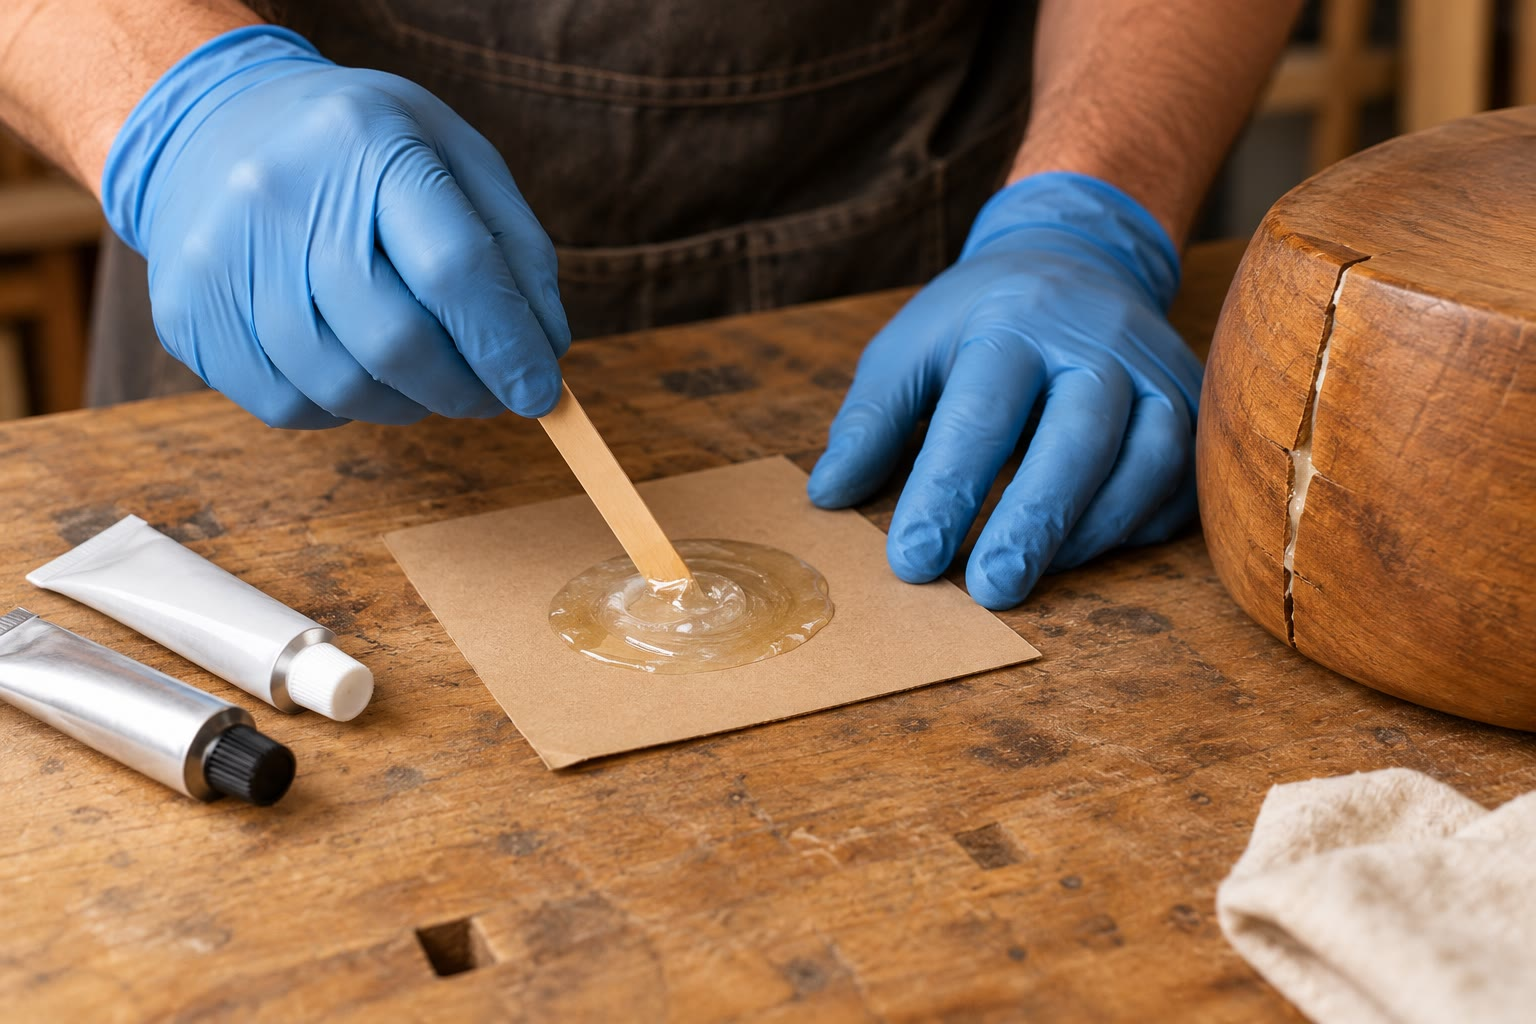
\includegraphics[width=0.6\linewidth]{images/book3/ai/b2-21-epoxy.jpg}

{\small Mencampur lem epoksi dua komponen: resin, yang mengandung gugus
\omterm{def:b2:alkene-redox:epoxide}{epoksida}, dan pengeras, sebuah amina, bereaksi begitu keduanya bertemu;
cincin-cincin itu terbuka dan menautkan molekul-molekul menjadi jaringan
padat.}
\end{omfigure}

\section{Hidrogenasi katalitik}

\begin{definition}[Hidrogenasi katalitik]\label{def:b2:alkene-redox:hydrogenation}
Yang disebut \emph{hidrogenasi katalitik}\index{hidrogenasi katalitik}
menambahkan dihidrogen pada ikatan rangkap dengan adanya katalis: logam
yang terbagi halus (paladium pada karbon, platina, nikel) dalam katalisis
heterogen, atau kompleks yang larut seperti katalis Wilkinson dalam
katalisis homogen.
\end{definition}

Pada permukaan logam, dihidrogen dan alkena sama-sama tertahan, ikatan
\ce{H-H} terputus menjadi atom-atom hidrogen permukaan, dan atom-atom ini
dipindahkan satu demi satu ke atom-atom karbon alkena, yang terbaring datar
di atas logam.

\begin{proposition}[Adisi sin]\label{prop:b2:alkene-redox:syn-hydrogenation}
\omterm{def:b2:alkene-redox:hydrogenation}{Hidrogenasi katalitik} mengantarkan kedua atom hidrogen ke muka yang sama
dari ikatan rangkap. Alkuna yang dihidrogenasi dengan katalis paladium yang
diracuni berhenti pada alkena, yaitu isomer
(\textit{Z}).
\end{proposition}

\begin{proof}[Argumen]
Alkena terikat pada katalis melalui satu mukanya, dan kedua hidrogen
berasal dari katalis, pada muka itu: adisi sin. Pada alkuna, kedua hidrogen
yang diadisikan pada ikatan rangkap tiga berada pada sisi yang sama, saling
cis: alkena (\textit{Z}). Katalis yang sebagian dinonaktifkan (paladium pada
kalsium karbonat dengan garam timbal dan kuinolina) mengikat alkuna jauh
lebih kuat daripada alkena yang terbentuk, sehingga alkena itu meninggalkan
permukaan sebelum terjadi adisi kedua.
\end{proof}

\section{Hidroborasi--oksidasi}

\begin{definition}[Hidroborasi]\label{def:b2:alkene-redox:hydroboration}
Yang disebut \emph{hidroborasi}\index{hidroborasi} menambahkan ikatan B--H
sebuah boran pada ikatan \ce{C=C}; jika diikuti oleh oksidasi dengan
hidrogen peroksida basa, reaksi ini mengubah alkena menjadi alkohol yang
gugus hidroksilnya terletak pada karbon yang kurang tersubstitusi:
\emph{orientasi anti-Markovnikov}\index{orientasi anti-Markovnikov}.
\end{definition}

\begin{omfigure}
\setchemfig{atom sep=1.8em}
\schemestart[][west]
\chemfig{H_3C-[:30]CH=[:-30]CH_2}
\+ \chemfig{H-BH_2}
\arrow{->[adisi sin]}
\chemfig{H_3C-[:30]CH_2-[:-30]CH_2-[:30]BH_2}
\arrow{->[\ce{H2O2}][\ce{HO-}]}
\chemfig{H_3C-[:30]CH_2-[:-30]CH_2-[:30]OH}
\schemestop
\par\vspace{6pt}

{\small Hidroborasi--oksidasi propena. Boran beradisi dalam satu tahap,
boron pada karbon ujung dan hidrogen pada karbon dalam, keduanya pada muka
yang sama; oksidasi menggantikan boron dengan \ce{OH} dengan retensi
konfigurasi. Yang terbentuk adalah propan-1-ol, bukan propan-2-ol hasil
hidrasi terkatalisis asam.}
\end{omfigure}

\begin{proposition}[Orientasi hidroborasi]\label{prop:b2:alkene-redox:hydroboration-regio}
Boron beradisi pada karbon ikatan rangkap yang kurang tersubstitusi, dan
hidrogen pada karbon yang lebih tersubstitusi; adisinya sin.
\end{proposition}

\begin{proof}[Argumen]
Boron, dengan orbital p yang kosong, adalah elektrofilnya: dalam keadaan
transisi empat pusat (kedua karbon, boron, dan hidrogen), ikatan dengan
boron terbentuk sedikit lebih dahulu daripada ikatan C--H, dan muatan
positif parsial berkembang pada karbon yang lain, yang lebih baik dipikul
oleh karbon yang lebih tersubstitusi; gugus boron yang meruah juga lebih
menyukai ujung yang kurang terhalang. Kedua ikatan baru terbentuk pada satu
muka, dalam satu tahap serempak: sin.
\end{proof}

\begin{proposition}[Oksidasi dengan retensi]\label{prop:b2:alkene-redox:retention}
Oksidasi alkilboran oleh hidrogen peroksida basa menggantikan setiap ikatan
C--B dengan ikatan C--OH dengan retensi konfigurasi pada karbon.
\end{proposition}

\begin{proof}[Argumen]
Anion hidroperoksida beradisi pada boron; sebuah gugus alkil lalu bermigrasi
dari boron ke oksigen di sebelahnya, bersama pasangan elektronnya, sementara
hidroksida pergi; karbonnya mempertahankan ikatan-ikatannya pada sisi yang
sama sepanjang proses itu. Hidrolisis ikatan B--O membebaskan alkoholnya.
\end{proof}

\section{Epoksida}

\begin{definition}[Epoksida]\label{def:b2:alkene-redox:epoxide}
Yang disebut \emph{epoksida}\index{epoksida} (oksirana) adalah eter siklik
dengan cincin beranggota tiga yang terdiri atas dua karbon dan satu oksigen.
\emph{Epoksidasi}\index{epoksidasi} mengubah alkena menjadi epoksida,
biasanya dengan sebuah \emph{asam peroksi}\index{asam peroksi} \ce{RCO3H}, yang
memindahkan satu atom oksigen ke ikatan rangkap.
\end{definition}

\begin{omfigure}
\setchemfig{atom sep=2em}
\schemestart
\chemfig{R-[:30]CH=[:-30]CH-[:30]R}
\+ \chemfig{Ar-C(=[2]O)-O-O-H}
\arrow{->}
\chemfig{[:-60]CH(-[:210]R)*3(-CH(-[:-30]R)-O-)}
\+ \chemfig{Ar-C(=[2]O)-OH}
\schemestop
\par\vspace{6pt}

{\small \omterm{def:b2:alkene-redox:epoxide}{Epoksidasi} oleh \omterm{def:b2:alkene-redox:epoxide}{asam peroksi} (Ar: misalnya gugus 3-klorofenil).
Oksigen ujung \omterm{def:b2:alkene-redox:epoxide}{asam peroksi} dipindahkan ke ikatan rangkap dalam satu tahap,
dengan kedua ikatan C--O terbentuk pada muka yang sama.}
\end{omfigure}

\begin{proposition}[Epoksidasi stereospesifik]\label{prop:b2:alkene-redox:epoxidation}
\omterm{def:b2:alkene-redox:epoxide}{Epoksidasi} oleh \omterm{def:b2:alkene-redox:epoxide}{asam peroksi} bersifat stereospesifik: alkena (\textit{Z})
menghasilkan \omterm{def:b2:alkene-redox:epoxide}{epoksida} cis, alkena (\textit{E}) menghasilkan \omterm{def:b2:alkene-redox:epoxide}{epoksida} trans.
\end{proposition}

\begin{proof}
Oksigen dipindahkan dalam satu tahap serempak ke satu muka ikatan rangkap,
yang sementara itu tidak berotasi: posisi relatif substituen-substituennya
dipertahankan.
\end{proof}

\begin{proposition}[Pembukaan epoksida]\label{prop:b2:alkene-redox:opening}
Nukleofil membuka \omterm{def:b2:alkene-redox:epoxide}{epoksida} dengan menyerang salah satu karbon dari muka yang
berseberangan dengan oksigen (pembukaan anti, dengan inversi pada karbon
itu). Dalam kondisi basa, nukleofil menyerang karbon yang kurang
terhalang; dalam kondisi asam, karbon yang lebih tersubstitusi.
\end{proposition}

\begin{proof}[Argumen]
Tegangan cincin membuat ikatan-ikatan C--O mudah diputus. Dengan nukleofil
kuat dan tanpa asam, pembukaannya merupakan substitusi bimolekular, dan
karbon yang paling kurang terhalang paling mudah dicapai. Dalam asam,
oksigennya terprotonasi; ikatan C--O ke karbon yang lebih tersubstitusi
paling teregang, karena karbon itu memikul muatan positif parsial yang lebih
besar, dan bahkan nukleofil lemah (air, alkohol) menyerang di sana ---
tetap dari belakang, jadi tetap anti.
\end{proof}

\begin{omfigure}
\setchemfig{atom sep=2em}
\schemestart
\chemfig{[:-60]C(-[:210]H_3C)(-[:150]H_3C)*3(-CH_2-O-)}
\arrow{->[\ce{CH3O-}][\ce{CH3OH}]}[,1.4]
\chemfig{H_3C-C(-[2]CH_3)(-[6]OH)-CH_2-OCH_3}
\schemestop

\medskip
\schemestart
\chemfig{[:-60]C(-[:210]H_3C)(-[:150]H_3C)*3(-CH_2-O-)}
\arrow{->[\ce{CH3OH}][\ce{H+}]}[,1.4]
\chemfig{H_3C-C(-[2]CH_3)(-[6]OCH_3)-CH_2-OH}
\schemestop
\par\vspace{6pt}

{\small Pembukaan 2,2-dimetiloksirana oleh metanol. Atas, dengan metoksida:
serangan pada \ce{CH2}, karbon yang kurang terhalang. Bawah, dalam asam:
serangan pada karbon yang lebih tersubstitusi, yang memikul sebagian besar
muatan positif \omterm{def:b2:alkene-redox:epoxide}{epoksida} yang terprotonasi.}
\end{omfigure}

\section{Dihidroksilasi}

\begin{definition}[Dihidroksilasi]\label{def:b2:alkene-redox:dihydroxylation}
Yang disebut \emph{dihidroksilasi}\index{dihidroksilasi} mengubah alkena
menjadi 1,2-diol dengan menambahkan satu gugus \ce{OH} pada setiap karbon
ikatan rangkap.
\end{definition}

Osmium tetroksida, dalam jumlah katalitik bersama pengoksidasi ulang, dan
permanganat encer dingin menambahkan kedua oksigen melalui sebuah ester
siklik, pada satu muka: \omterm{def:b2:alkene-redox:dihydroxylation}{dihidroksilasi} sin. \omterm{def:b2:alkene-redox:epoxide}{Epoksidasi} yang diikuti oleh
pembukaan dengan air dalam asam menghasilkan diol anti.

\begin{proposition}[Diol sin dan anti]\label{prop:b2:alkene-redox:diols}
Dari (\textit{Z})-but-2-ena, \omterm{def:b2:alkene-redox:dihydroxylation}{dihidroksilasi} sin menghasilkan
meso-butana-2,3-diol dan jalur \omterm{def:b2:alkene-redox:epoxide}{epoksida} menghasilkan diol-diol rasemat
(2\textit{R},3\textit{R}) dan (2\textit{S},3\textit{S}); dari
(\textit{E})-but-2-ena, hasil-hasilnya bertukar.
\end{proposition}

\begin{proof}
Dalam (\textit{Z})-but-2-ena kedua metil berada pada sisi yang sama.
Menambahkan dua \ce{OH} pada satu muka menghasilkan diol yang, jika
digambarkan dalam konformasi eklips bekas ikatan rangkap, kedua \ce{OH}-nya
berada pada satu sisi dan kedua metilnya pada sisi yang lain: sebuah bidang
cermin melalui tengah-tengah C2 dan C3, yaitu senyawa meso. Jalur \omterm{def:b2:alkene-redox:epoxide}{epoksida}
menempatkan kedua \ce{OH} pada muka yang berseberangan (anti): bidang cermin
itu hilang, dan serangan pada salah satu karbon \omterm{def:b2:alkene-redox:epoxide}{epoksida} yang akiral itu,
yang sama-sama mungkin, menghasilkan kedua enansiomer dalam jumlah yang
sama. Untuk alkena (\textit{E}), setiap tahap mengubah hubungan antara
kedua metil, sehingga hasil-hasilnya bertukar.
\end{proof}

\begin{omfigure}
\begin{tikzpicture}[font=\small]
  \begin{scope}
    \draw[thick] (0,0) -- (0,1.2);
    \draw[thick] (0,1.2) -- (-0.7,1.45); \draw[thick] (0,1.2) -- (0.7,1.45);
    \node[anchor=east] at (-0.7,1.45) {\ce{HO}}; \node[anchor=west] at (0.7,1.45) {\ce{CH3}};
    \draw[thick] (0,0) -- (-0.7,0.25); \draw[thick] (0,0) -- (0.7,0.25);
    \node[anchor=east] at (-0.7,0.25) {\ce{HO}}; \node[anchor=west] at (0.7,0.25) {\ce{CH3}};
    \node[anchor=south] at (0,1.25) {\scriptsize H};
    \node[anchor=north] at (0,-0.05) {\scriptsize H};
    \draw[densely dashed, omThm] (-1.6,0.6) -- (1.6,0.6);
    \node at (0,-1.0) {sin: meso};
  \end{scope}
  \begin{scope}[xshift=6.5cm]
    \draw[thick] (0,0) -- (0,1.2);
    \draw[thick] (0,1.2) -- (-0.7,1.45); \draw[thick] (0,1.2) -- (0.7,1.45);
    \node[anchor=east] at (-0.7,1.45) {\ce{HO}}; \node[anchor=west] at (0.7,1.45) {\ce{CH3}};
    \draw[thick] (0,0) -- (-0.7,0.25); \draw[thick] (0,0) -- (0.7,0.25);
    \node[anchor=east] at (-0.7,0.25) {\ce{H3C}}; \node[anchor=west] at (0.7,0.25) {\ce{OH}};
    \node[anchor=south] at (0,1.25) {\scriptsize H};
    \node[anchor=north] at (0,-0.05) {\scriptsize H};
    \node[align=center] at (0,-1.1) {anti: satu enansiomer\\ (terbentuk bersama bayangan cerminnya)};
  \end{scope}
\end{tikzpicture}

{\small Kedua butana-2,3-diol dari (\textit{Z})-but-2-ena, skematis (ikatan
C2--C3 tegak, kedua gugus setiap karbon digambar di kiri dan kanan). Adisi
sin menempatkan kedua \ce{OH} pada sisi yang sama: ada bidang cermin dalam
(putus-putus), yaitu senyawa meso. Adisi anti menempatkan keduanya pada sisi
yang berseberangan: diol kiral, yang terbentuk bersama enansiomernya.}
\end{omfigure}

\section{Pemutusan oksidatif}

\begin{definition}[Pemutusan oksidatif]\label{def:b2:alkene-redox:cleavage}
Yang disebut \emph{pemutusan oksidatif}\index{pemutusan oksidatif} memutus
kedua ikatan dari ikatan rangkap \ce{C=C} dan mengubah setiap karbonnya
menjadi gugus karbonil atau karboksil. Dalam
\emph{ozonolisis}\index{ozonolisis}, alkena bereaksi dengan ozon dan ozonida
antaranya diuraikan dalam tahap kedua, yaitu tahap pengolahan.
\end{definition}

\begin{proposition}[Produk ozonolisis]\label{prop:b2:alkene-redox:ozonolysis}
\omterm{def:b2:alkene-redox:cleavage}{Ozonolisis} memecah setiap ikatan \ce{C=C} menjadi dua gugus \ce{C=O}. Dengan
pengolahan reduktif (seng dan asam, atau dimetil sulfida), karbon yang
membawa hidrogen menghasilkan aldehida; dengan pengolahan oksidatif
(hidrogen peroksida), karbon itu menghasilkan asam karboksilat. Karbon yang
membawa dua gugus karbon menghasilkan keton dalam kedua kasus.
\end{proposition}

\begin{proof}[Argumen]
Ozon beradisi pada ikatan rangkap, zat antaranya mengalami penataan ulang dan
ikatan C--C terputus, sehingga terbentuk ozonida yang setiap bekas karbon
alkenanya terikat pada dua oksigen. Tahap pengolahan mereduksinya menjadi dua
senyawa karbonil, atau mengoksidasi aldehida-aldehidanya lebih lanjut.
Tahap-tahap antaranya diterima tanpa bukti.
\end{proof}

\begin{omfigure}
\setchemfig{atom sep=2em}
\schemestart
\chemfig{H_3C-[:30]C(-[:90]CH_3)=[:-30]CH-[:30]CH_3}
\arrow{->[1. \ce{O3}][2. \ce{Zn}, \ce{H+}]}[,1.8]
\chemfig{H_3C-C(=[2]O)-CH_3}
\+
\chemfig{H-C(=[2]O)-CH_3}
\schemestop
\par\vspace{6pt}

{\small \omterm{def:b2:alkene-redox:cleavage}{Ozonolisis} 2-metilbut-2-ena dengan pengolahan reduktif: propanon dan
etanal. Menyambungkan kembali kedua karbon karbonil dengan ikatan rangkap
membangun kembali alkenanya.}
\end{omfigure}

\begin{method}[Menentukan letak ikatan rangkap]\label{met:b2:alkene-redox:locate-double-bond}
\begin{enumerate}
  \item Daftarlah fragmen-fragmen karbonil hasil \omterm{def:b2:alkene-redox:cleavage}{ozonolisis} dan hitunglah
        karbonnya; jumlahnya harus sama dengan jumlah karbon alkena.
  \item Setiap karbon \ce{C=O} dulunya adalah karbon berikatan rangkap:
        sambungkan fragmen-fragmennya dengan menggantikan dua
        \ce{C=O} dengan satu \ce{C=C}.
  \item Untuk sebuah cincin, yang keluar adalah satu molekul dengan dua gugus
        karbonil; sambungkan kedua ujungnya.
  \item Periksalah dengan rumus dan derajat ketidakjenuhannya.
\end{enumerate}
\end{method}

Permanganat pekat panas juga memutus ikatan rangkap, dengan menghasilkan
asam dan keton; natrium periodat memutus 1,2-diol menjadi dua senyawa
karbonil, jalur yang lebih lunak melalui diol.

\begin{method}[Memilih pereaksi untuk alkena]\label{met:b2:alkene-redox:choose-reagent}
\begin{center}
\small
\renewcommand{\arraystretch}{1.15}
\begin{tabular}{lll}
sasaran & pereaksi & stereokimia, orientasi \\ \hline
alkana & \ce{H2}, Pd/C & sin \\
alkohol Markovnikov & \ce{H2O}, asam & melalui karbokation \\
alkohol anti-Markovnikov & \ce{BH3}, lalu \ce{H2O2}, \ce{HO-} & sin \\
\omterm{def:b2:alkene-redox:epoxide}{epoksida} & \omterm{def:b2:alkene-redox:epoxide}{asam peroksi} & stereospesifik \\
diol sin & \ce{OsO4} (kat.) atau \ce{MnO4-} dingin & sin \\
diol anti & \omterm{def:b2:alkene-redox:epoxide}{asam peroksi}, lalu \ce{H2O}, asam & anti \\
dua karbonil & \ce{O3}, lalu \ce{Zn}/asam & pemutusan \\
\end{tabular}
\end{center}
\end{method}

\begin{safety}{\ghs[5mm]{GHS02}\,\ghs[5mm]{GHS03}\,\ghs[5mm]{GHS05}\,\ghs[5mm]{GHS06}}
Osmium tetroksida mudah menguap dan sangat beracun (merusak mata); senyawa
ini dipakai dalam jumlah katalitik dalam larutan, di dalam lemari asam. \omterm{def:b2:alkene-redox:epoxide}{Asam
peroksi} dan hidrogen peroksida adalah pengoksidasi yang dapat terurai dengan
hebat jika dipanaskan atau dipekatkan; larutan boran mudah terbakar; ozon
beracun dan dibangkitkan di dalam lemari asam.
% ledger: ghs:OsO4, ghs:mCPBA, ghs:BH3-THF, ghs:O3, ghs:NaIO4
\end{safety}

\section{Latihan}

\begin{exercise}[$\star$]\label{exo:b2:alkene-redox:1}
Tuliskan produk 1-metilsikloheksena dengan: \ce{H2}/Pd; \ce{H2O}/\ce{H+};
\ce{BH3} lalu \ce{H2O2}/\ce{HO-}; \omterm{def:b2:alkene-redox:epoxide}{asam peroksi}; \ce{OsO4} (kat.); \ce{O3} lalu
\ce{Zn}/\ce{H+}.
\end{exercise}

\begin{exercise}[$\star$]\label{exo:b2:alkene-redox:2}
Alkohol manakah yang dihasilkan hidroborasi--oksidasi dari 2-metilpropena?
Dan hidrasi terkatalisis asam?
\end{exercise}

\begin{exercise}[$\star$]\label{exo:b2:alkene-redox:3}
Gambarlah \omterm{def:b2:alkene-redox:epoxide}{epoksida} yang terbentuk dari (\textit{E})-but-2-ena. Apakah \omterm{def:b2:alkene-redox:epoxide}{epoksida} itu kiral?
\end{exercise}

\begin{exercise}[$\star$]\label{exo:b2:alkene-redox:4}
Tuliskan produk-produk \omterm{def:b2:alkene-redox:cleavage}{ozonolisis} heks-3-ena dengan pengolahan reduktif,
lalu dengan pengolahan oksidatif.
\end{exercise}

\begin{exercise}[$\star\star$]\label{exo:b2:alkene-redox:5}
Tuliskan diol-diol yang terbentuk dari (\textit{Z})-but-2-ena (a) dengan
\ce{OsO4}; (b) dengan \omterm{def:b2:alkene-redox:epoxide}{asam peroksi} lalu asam berair. Manakah yang tidak
aktif secara optik karena merupakan senyawa meso, dan manakah yang karena
rasemat?
\end{exercise}

\begin{exercise}[$\star\star$]\label{exo:b2:alkene-redox:6}
2,2-Dimetiloksirana dibuka oleh air dalam asam dan oleh hidroksida. Apakah
kedua jalur itu menghasilkan produk yang sama? Jelaskan.
\end{exercise}

\begin{exercise}[$\star\star$]\label{exo:b2:alkene-redox:7}
Bagaimana (\textit{Z})-heks-3-ena dapat dibuat dari heks-3-una?
\end{exercise}

\begin{exercise}[$\star\star$]\label{exo:b2:alkene-redox:8}
Sebuah alkena \ce{C7H14} menghasilkan, melalui \omterm{def:b2:alkene-redox:cleavage}{ozonolisis} dengan pengolahan
reduktif, propanon dan butanal. Tentukan strukturnya.
\end{exercise}

\begin{exercise}[$\star\star$]\label{exo:b2:alkene-redox:9}
Usulkan sintesis heksan-1-ol dari heks-1-ena, dan jelaskan mengapa hidrasi
terkatalisis asam akan gagal.
\end{exercise}

\begin{exercise}[$\star\star\star$]\label{exo:b2:alkene-redox:10}
Limonena mempunyai ikatan rangkap cincin yang trisubstitusi dan ikatan
rangkap eksosiklik yang disubstitusi (\ce{C(CH3)=CH2}). Manakah yang lebih
dahulu bereaksi dengan satu ekuivalen \omterm{def:b2:alkene-redox:epoxide}{asam peroksi}, dan manakah dengan satu
ekuivalen boran yang meruah? Jelaskan.
\end{exercise}

\begin{exercise}[$\star\star\star$]\label{exo:b2:alkene-redox:11}
Buatlah trans-sikloheksana-1,2-diol dan cis-sikloheksana-1,2-diol dari sikloheksena.
\end{exercise}

\begin{exercise}[$\star\star\star$]\label{exo:b2:alkene-redox:12}
Sebuah senyawa \ce{C6H10} menyerap satu ekuivalen \ce{H2}. \omterm{def:b2:alkene-redox:cleavage}{Ozonolisisnya}
dengan pengolahan reduktif menghasilkan satu produk saja, heksanadial
\ce{OHC-(CH2)4-CHO}. Identifikasilah senyawa itu.
\end{exercise}

\section{Soal: Mengidentifikasi Sebuah Terpena}

\begin{problem}[{Soal akhir pekan --- rumus dan ketidakjenuhan limonena,
hidrogenasinya, fragmen-fragmen ozonolisisnya, dan reaksi-reaksi selektif
kedua ikatan rangkapnya}]
\label{pb:b2:alkene-redox:1}
Limonena, aroma kulit jeruk, mempunyai rumus \ce{C10H16}. Senyawa ini adalah
1-metil-4-(prop-1-en-2-il)sikloheks-1-ena: sebuah ikatan rangkap cincin yang
membawa metil, dan gugus eksosiklik \ce{C(CH3)=CH2} pada karbon cincin yang
berseberangan. $R =
\qty{8.314}{J/(K.mol)}$; massa molar (\unit{g/mol}): C 12.011, H 1.008.
% ledger: aw:C, aw:H, const:R, ghs:limonene

\medskip
\noindent\textbf{Bagian I --- Rumus dan hidrogenasi.}
\begin{enumerate}
  \item Hitunglah massa molar limonena.
  \item Hitunglah derajat ketidakjenuhannya.
  \item Berapa cincin dan berapa ikatan rangkap yang dimilikinya?
  \item Tuliskan hidrogenasinya dengan paladium, termasuk produknya.
  \item Hitunglah jumlah dihidrogen yang diserap oleh \qty{1.00}{g} limonena.
  \item Hitunglah volumenya pada \qty{25}{\degreeCelsius} dan \qty{1.00}{bar}.
  \item Apakah produknya kiral?
\end{enumerate}

\medskip
\noindent\textbf{Bagian II --- \omterm{def:b2:alkene-redox:cleavage}{Ozonolisis}.}
\begin{enumerate}[resume]
  \item Fragmen-fragmen apakah yang dihasilkan \omterm{def:b2:alkene-redox:cleavage}{ozonolisis} dengan pengolahan
        reduktif? (Hitunglah karbonnya.)
  \item Mengapa ikatan rangkap cincin menghasilkan satu molekul, bukan dua?
  \item Fragmen manakah yang hilang sebagai gas atau cairan yang mudah menguap?
  \item Bagaimana produk-produknya akan berbeda dengan pengolahan oksidatif?
  \item Tunjukkan bagaimana fragmen-fragmen itu menentukan letak kedua ikatan rangkap.
  \item Berapa pusat stereogenik yang dimiliki limonena, dan apakah \omterm{def:b2:alkene-redox:cleavage}{ozonolisis}
        mempertahankannya?
\end{enumerate}

\medskip
\noindent\textbf{Bagian III --- \omterm{def:b2:alkene-redox:hydroboration}{Hidroborasi}.}
\begin{enumerate}[resume]
  \item Dengan satu ekuivalen boran yang meruah, ikatan rangkap manakah yang
        bereaksi? Mengapa?
  \item Gambarlah produknya setelah oksidasi.
  \item Apakah alkohol yang baru itu primer, sekunder, atau tersier?
  \item Mengapa orientasinya disebut anti-Markovnikov?
  \item Berapa stereoisomer yang dapat terbentuk pada pusat stereogenik yang baru?
  \item Pereaksi manakah yang sebaliknya akan menempatkan \ce{OH} pada karbon
        yang lebih tersubstitusi dari ikatan rangkap yang
        sama?
\end{enumerate}

\medskip
\noindent\textbf{Bagian IV --- \omterm{def:b2:alkene-redox:epoxide}{Epoksidasi}.}
\begin{enumerate}[resume]
  \item Dengan satu ekuivalen \omterm{def:b2:alkene-redox:epoxide}{asam peroksi}, ikatan rangkap manakah yang
        bereaksi? Mengapa?
  \item Gambarlah \omterm{def:b2:alkene-redox:epoxide}{epoksidanya}.
  \item Bukalah \omterm{def:b2:alkene-redox:epoxide}{epoksida} itu dengan air dalam asam: pada karbon manakah air menyerang?
  \item Gambarlah diolnya dan tentukan orientasi relatif kedua \ce{OH}-nya.
  \item Bagaimana diastereomer yang lain dari diol ini dapat diperoleh?
  \item Nyatakan volume dihidrogen yang diserap oleh \qty{1.00}{g} limonena pada
        \qty{25}{\degreeCelsius} dan \qty{1}{bar}.
\end{enumerate}
\end{problem}
